\documentclass[../../main/main.tex]{subfiles}
\begin{document}
\section{Introduction}


\subsection{Poker Concepts}

This paper references many general concepts from poker including bluffing, value betting, ranges, and pot odds. This section provides a brief overview of these concepts and how they are related.

There are many variants of poker, but all of them include central concepts which make the games strategically similar. Clearly, every decision a player makes in poker is dependent on their own hand strength and their perception of their opponent's hand strength. 

In nearly every poker variant, there are two reasons for a player to bet: when you want the opponent to call, and when you want the opponent to fold. In the first case, you may want the opponent to call because you expect to win the pot and want it to be larger. In the second case, you may want the opponent to fold because you believe you have a losing hand. This first case is called \textit{value betting}, and the second case is called \textit{bluffing}. The actions may look exactly the same to the opponent, but are distinguished by the intention of the bettor. For this reason, value bets are generally made strong hands and bluffs with weak ones.

The second important concept is \textit{ranges}. A range in poker refers to the possible hands or hand strengths that a player could have, conditioned on the actions they have taken and their strategy. A player's range is initially relevant to the opponent, but can also be used to describe how a player chooses their strategy. Following from this, a \textit{value range} refers to the range of hands that a player value bets with, and a \textit{bluffing range} refers to the range of hands that a player bluffs with. A \textit{weighted range} is a probability distribution over a range describing the probability that a player has any given hand strength, conditioned on their past actions. In real games, this concept can be somewhat nebulous, since real players' strategies change over time (often intentionally to confuse their opponent). However, in the context of Nash Equilibria, we can make this concept precise because the strategies are fixed and well-defined. In Nash Equilibrium, we can assume that each player knows their opponent's weighted range exactly and plays optimally given that knowledge. 

The third important concept is \textit{pot odds}. Pot odds are the ratio of the pot size to the amount a player must put in to call. In poker, the pot odds are often used to determine whether a player should call or fold. For example, if the pot is 100 and the player must bet 20 to call, the pot odds are 5:1. This means that the player should call if they believe they have a better than 1/6 chance of winning the pot. Higher pot odds make a call more appealing and lower pot odds make a call less appealing, given the same probability of winning. 

\subsection{Previous Work}

\subsubsection{Fixed-Bet Continuous Poker (FBCP)}

Continuous Poker (also called Von Neumann Poker, and referred to in this paper as Fixed-Bet Continuous Poker or FBCP) is a simplified model of poker. It is a two-player zero-sum game designed to study strategic decision-making in competitive environments. The game abstracts away many complexities of real poker, focusing instead on the mathematical and strategic aspects of bluffing, betting, and optimal play.

\begin{definition}[FBCP]
Two players, referred to as the bettor and the caller, each put a 0.5 unit ante into a pot\footnote{An ante of 1 is often used, but since the pot size is the more relevant value, we use an ante of 0.5. All bet sizes simply scale proportionally.}. They are each dealt a `hand strength' uniformly and independently from the interval $[0, 1]$ (referred to as $x$ for bettor and $y$ for caller). After seeing $x$, the bettor can either check - in which case, the higher hand between $x$ and $y$ wins the pot of 1 and the game ends - or they can bet by putting a pre-determined amount $B > 0$ into the pot. The caller can now either call by matching the bet of $B$, after which the higher hand wins the pot of $1+2B$, or fold, conceding the pot of $1+B$ to the bettor and ending the game.
\end{definition}

FBCP has many Nash equilibria, but it has a unique one in which the caller plays an admissible strategy\footnote{An admissible strategy is one which is not strictly dominated by any other strategy.}, as shown by Ferguson and Ferguson \cite[p. 2]{ferguson2003borel}. This strategy profile, parametrized by the bet size $B$, is as follows:

The bettor bets with hands $x$ such that either 

$$x > \frac{1 + 4B + 2B^2}{(1+2B)(2+B)} \text{ or } x < \frac{B}{(1+2B)(2+B)}$$

We call the higher interval the value betting range and the lower interval the bluffing range. The caller calls with hands $y$ above a calling threshold:

$$ y > \frac{B(3 +2B)}{(1+2B)(2+B)} $$

The non-uniqueness of this Nash Equilibrium is due to the fact that given the bettor's strategy, the caller can achieve the same expected payoff with any calling threshold between the value betting threshold and the bluffing threshold. However, any calling strategy other than this one incentivizes the bettor to deviate from the Nash Equilibrium strategy and leads to a lower payoff for the caller after two deviations. 

The value of FBCP for the bettor is 

$$ V_{FB}(B) = \frac{B}{2(1+2B)(2+B)} $$

Which is positive (advantageous to the bettor) and maximized at $B = 1$, when the bet size is exactly the pot size. 

\subsubsection{No-limit Continuous Poker (NLCP)}
Another continuous poker variant allows the bettor to choose a bet size $s > 0$ after seeing their hand strength, as opposed to a fixed bet size $B$. This variant is called No-Limit Continuous Poker (or Newman Poker after Donald J. Newman, or NLCP in this paper). The Nash equilibrium strategy profile for this variant is discussed and solved by Bill Chen and Jerrod Ankenman \cite[p. 154]{chen2006mathematics}.

In Nash Equilibrium, the bettor should make large bets with their strongest and weakest hands and smaller bets or checks with their intermediate hands. It turns out that the optimal strategy is most elegantly described by a mapping from bet sizes $s$ to hand strengths $x$ for bluffing and value betting, respectively\footnote{This feels backwards - mapping hand strengths to bet sizes would be more natural, but the math is more elegant this way.}. The caller simply has a calling threshold $c(s)$ for each possible bet size $s$. The full strategy profile is as follows:

The bettor bets $s$ with hands $x$ such that either

$$ x = \frac{3 s+1}{7 (s+1)^3} \text{ or } x = 1 - \frac{3}{7 (s+1)^2} $$

Where the first condition represents bluffing hands and the second value betting hands. After seeing a bet of size $s$, the caller should call with hands $y$ such that

$$ y > 1 - \frac{6}{7 (s+1)} $$

See Figure \ref{fig:nlcp_strategy_profile} for a graphical representation of the strategy profile.

\begin{figure}[h!]
    \centering
    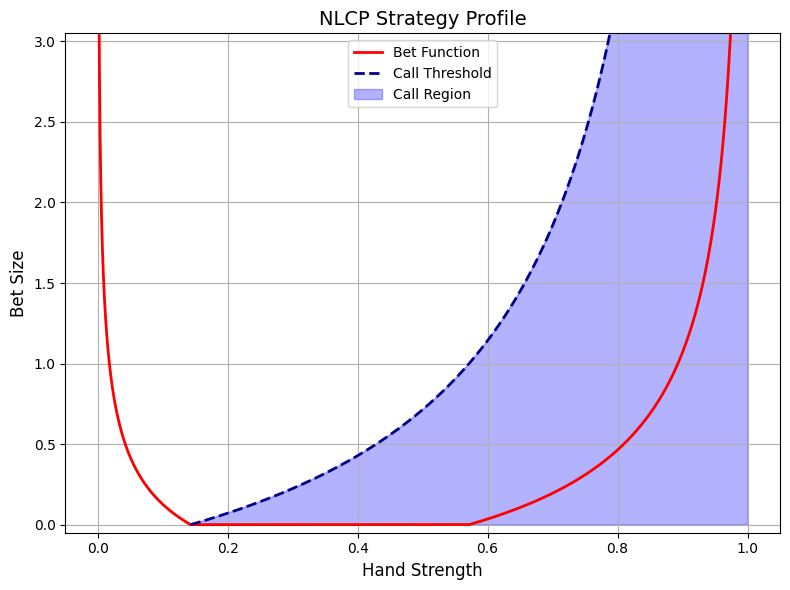
\includegraphics[width=0.8\textwidth]{images/NLCP_strategy_profile.png}
    \caption{NLCP Strategy Profile}
    \label{fig:nlcp_strategy_profile}
\end{figure}

Note that the bettor uses all possible bet sizes and has exactly two hand strengths for each bet size\footnote{Seen visually in Figure \ref{fig:nlcp_strategy_profile} by the fact that a horizontal line intersects the bet function at exactly two points.}. On first inspection, this feels like the bettor is giving away too much information, but it turns out to still an optimal strategy. This concept appears again and is explained more thoroughly in section \ref{subsec:nash_equilibrium_structure}.

The value of NLCP is

$$ V_{NL} = \frac{1}{14} $$

for the bettor\footnote{Would be 1/7 for an ante of 1, but the value is halved with an ante of 0.5.}. Thus, NLCP is again advantageous to the bettor. In fact, one can easily verify that NLCP is more advantageous to the bettor than FBCP for any bet size $B$ by arguing that the bettor could artificially restrict themselves to a single bet size and achieve the same value as the bettor in FBCP.
\end{document}